

% This is a simple sample document.  For more complicated documents take a look in the exercise tab. Note that everything that comes after a % symbol is treated as comment and ignored when the code is compiled.

\documentclass{article} % \documentclass{} is the first command in any LaTeX code.  It is used to define what kind of document you are creating such as an article or a book, and begins the document preamble

\usepackage{amsmath} % \usepackage is a command that allows you to add functionality to your LaTeX code
\usepackage{graphicx}
\usepackage{float}
\usepackage[demo]{rotating}

\title{Master Thesis Proposal:\\A flow-aware multipath tunnel implementation based on AF\_XDP socket} % Sets article title
\author{Ba Que Le, B.Sc} % Sets authors name
% \date{\today} % Sets date for date compiled

% The preamble ends with the command \begin{document}
\begin{document} % All begin commands must be paired with an end command somewhere
\maketitle % creates title using information in preamble (title, author, date)

Network tunnels facilitate isolated communication between applications and their surrounding environment.
However, current tunneling solutions encounter several challenges: 1. They operate on a single line.
2. Certain solutions are overly complicated due to their large and outdated code base.
3. Many low-level implementations rely on unsafe kernel modules.
4. Upgrading bandwidth necessitates the purchase of costlier equipment.
5. Enhancing reliability leads to increased complexity at both the infrastructure and application levels.
\\

% 100 words max: What you are proposing.
I propose a multipath, low-level tunnel library based on AF\_XDP-eBPF technology, called MTX (Multipath Tunnel using XDP technology) as the topic for a Master Thesis in Computer Science.
The tunnel will have the following properties:
% - Multipath support by design: can work in aggregation mode, fail-over mode or Intelligence-mode to fullfil requirements of total bandwidth and resilence. 
% - High performance: The underlying connections of the tunnel are managed by AF\_XDP sockets. This family of native Linux socket uses eBPF technology to deliver network packet to application at line speed. This technology offers both performance and safety by allowing packets to be processed in isolated environment in kernel space.
% - Simplicity: The library handles all initiation and management tasks. Only the interfaces to the tunnel and configuration are exposed to the application. 
\begin{itemize}
    \item Built-in support for multipath: The tunnel is designed to function in aggregation mode, fail-over mode, or mix-mode to meet different requirements for total bandwidth and resilience.
    \item  High performance: The underlying connections are managed through AF\_XDP sockets. These sockets, based on eBPF technology, can deliver packets to applications at line speed. This technology ensures both high performance and safety by allowing packet processing in a secure, isolated environment within the kernel space.
    \item  Simplicity: The library handles all initiation and management tasks. The application is only exposed to the tunnel's interfaces and configuration options.
\end{itemize}

% 100 words max: how your solution differs from others
% The result of the project will be an open source library to abstract all the multipath details and management tasks from application.
% Most tunnel protocols don't support multiple underlying connection.
% Unlike multipath protocol MPTCP or SCTP that can only used by 1 application, the MTX offers the tunnel connection for multiple applications for simultainously usage.
% Each application can specify how its traffic flows will be handled: priority, line preference, ...
The outcome of this project provides a comprehensive abstraction where multipath details are hiden from applications.
The MTX library allows multiple applications to utilize the tunnel connection simultaneously, unlike multipath protocols such as MPTCP or SCTP which restrict to a single application.
This centralized management allows better coordinating and planing of system resources.
By providing diversed configuration based on the tunnel's multipath nature, each application can have the ability to specify how its traffic flows will be handled, for instance by priority or line preference. This flexibility empowers applications to have granular control over their traffic management within the tunnel.
\\

% 50 words max: Bullet points with objectives
The following objectives are planned:
% - Design a multipath protocol: header structure, rules for traffic aggregator and distributor.
% - Implement and packaging: the library will be written in C/C++ language for Linux OS.
% - Demenstration: a application will be built to demonstrate the tunnel's features, preferly an implementation of GPT-U protocol that are being used in communication between 5G's UPF and gNodeB.
\begin{itemize}
    \item Multipath protocol design: Creating a well-defined header structure and establishing logic for traffic aggregation and distribution within the tunnel.
    \item Implementation and packaging: The library will be developed in C/C++ programming languages for Linux system.
    \item Tunnel library: Create the MTX library that are capable of handling distributing and aggregating traffic over multiple lines for multiple applications simultainously. 
    Additionally, make configuration available to govern traffic on flow and packet levels.
    \item Demonstration: Ideally, an implementation of the GPT-U protocol will be built to showcase the features of the tunnel. The protocol is used in communication between 5G's UPF (User Plane Function) and gNodeB (gNB).
\end{itemize}
% 100 words max: Usage scenario in 5G.
% Network ingress and egress modules in 5G systems attracted my interest: large commercial systems have complex software stack that split and aggregate traffic over multiple high performance NICs using DPDK and SRIOV technologies. 
% Open source projects such as Open5GS (which is being used in TU Berlin AV's 5G testbed) can't afford such investment and thus suffers from throughput limitation.
% I see MTX library as an opportunity to:
% - offer a alternative to improving performance at low cost (both financial and complexity) for existing projects.
% - contribute to 5G open source community.

The motivation for this project originated from the ingress and egress modules within current deployed 5G systems. 
These modules in large commercial systems are supported by complex software stacks to aggregate traffic across multiple high-performance NICs using technologies like DPDK and SRIOV.
Open source projects such as Open5GS (is currently employed in TU Berlin AV's 5G testbed) face limitations in terms of throughput due to the lack of resources to invest in such infrastructure.
As such, MTX library could provide an alternative, impactful solution that can enhance performance for existing projects at a low cost, both in terms of finances and complexity. 
This is also an opportunity for the AV chair to contribute more to the 5G open source community.
\\

% 100 words max: What is expected as a result?
At the end of the project, the MTX library is expected to be an alternative to existing tunnel software that is easy to intergrate, fast and safe.
The tunnel can be bound to in form of memory buffer or TUN/TAP interface for maximum compability without introducing extra complexity.
Data center and high performance usage can benifit from MTX's horizontal scaling ability by combining lines.
Heterogeneous , flow-based traffic usage such as 5G's PDU protocol matches the MTX ability to specify traffic flows over multiple lines with different capabilities and characteristics.
This would not only improve the overall performance of the system but also provide extra support for system's stability and Application's quality of service.
\\


% \clearpage
The project is planed to finish in 6 months.
The complete version of the proposal will provide a more comprehensive introduction to the topic.

\begin{sidewaysfigure}
	\centering
	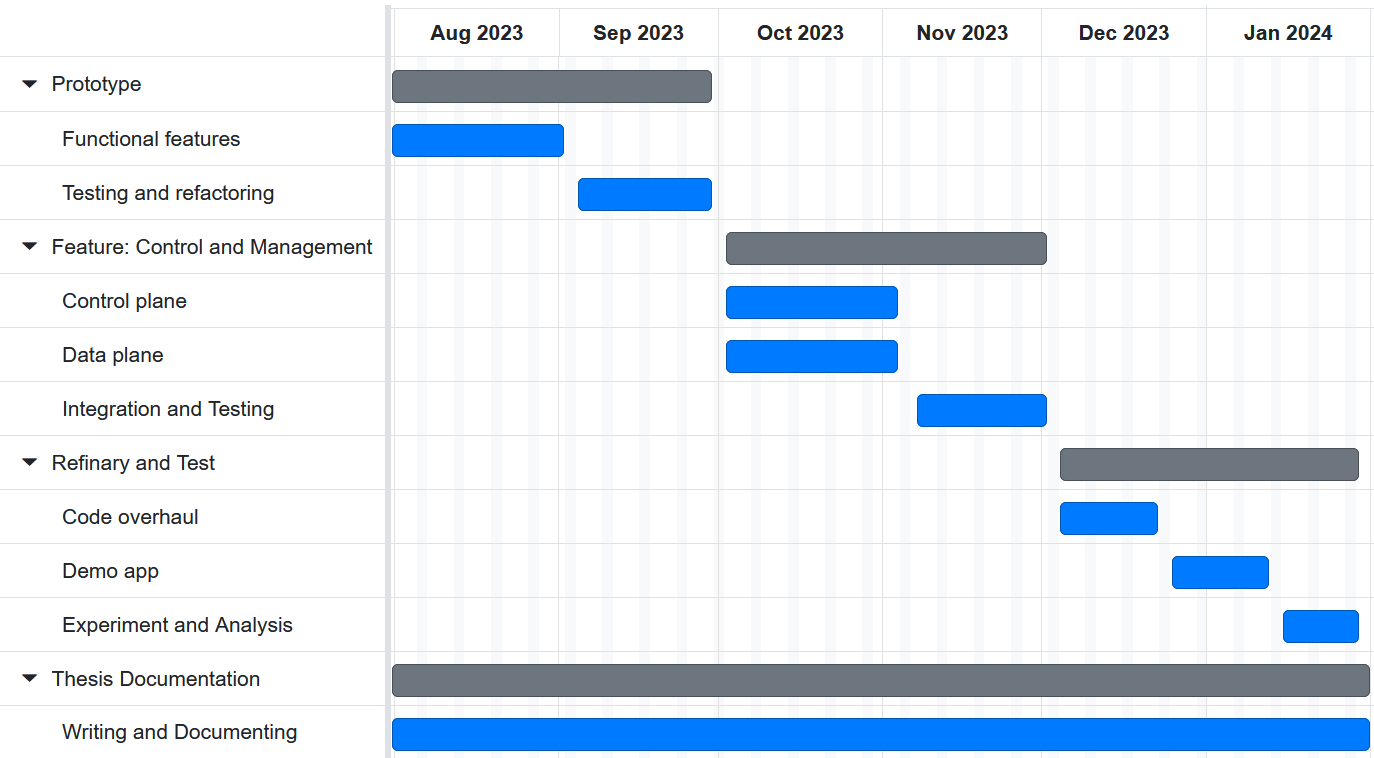
\includegraphics[width=1.0\textwidth]{resources/images/mini_gannt.PNG}
	\caption{GANTT chart: project progress plan}
\end{sidewaysfigure}


\end{document} % This is the end of the document


% Master Thesis Proposal: A flow-aware multipath tunnel implementation based on AF\_XDP socket

